\chapter{Implementation and experiments}  
\label{cha:android}

Nowadays the Android operative system is the most popular platform for
Smartphones and mobile devices. Due to this fact, there is a great interest in
the development of all sort of applications and with it, many tools have
been adapted to this platform for the use of the developers. One of these tools
is the OpenCV library for computer vision by \cite{opencv}.

This powerful library have already implemented the most common computer vision
algorithms and methods. In particular we can find the Machine Learning approach
for object detection in images explained in the previous
section~\ref{sec:objectdetec}.  It was perfectly suited by the implementation of this
project.

In this chapter is going to be presented the details about the Android
Application and the qualitative results on the performance of the application.

\section{The Android Application} % (fold)
\label{sec:androidapp}

In this section, the structure of the application is going to be presented. The
functionality of the main components is going to be explained aiming for future
improvements. In the figure~\ref{fig:andrivedir} is illustrated the directory
structure of the application.

\begin{figure}
    \centering\small
    \begin{minipage}[t]{0.6\linewidth}
        \dirtree{%
            .1 Andrive/. 
            .2 jni/. 
            .3 Android.mk. 
            .3 tum\_andrive\_DetectionBasedTracker.h.
            .3 detector\_native\_source.cpp.
            .2 src/. 
            .3 tum/.
            .4 andrive/.
            .5 Andrive.java.
            .5 GPSListener.java.
            .5 DetectionBasedTracker.java.
            .2 res/. 
            .3 raw/. 
            .4 cascade.xml. 
        }
    \end{minipage}
\caption{Directory structure of the Android application}
\label{fig:andrivedir}
\end{figure}

Maybe the most important file is the \textit{cascade.xml}. This file contains
the learned classifier used for image classification and vehicle detection. This
basically implies that it can be easily substituted by any other classifier for
either improving the classification or detect other objects.

Secondly, we have the source files under the \textit{src} directory. For the
vehicle detection module we have basically two files. The
\textit{DetectionBasedTracker.java} which defines the class with the same name.
This class implements the image classification task. It reads the
\textit{cascade.xml} file and use it to classified the images in the way
described in the chapter~\ref{kap:vehicle-detection}. The second file is the
\textit{GPSListener.java} which implements the class in charge of processing the
GPS signal and extract the speed for the calculation of the Time Headway
measurement (THM). 

Finally in the \textit{jni} directory are the native source files used by the
Java Native Interface (JNI). This native source is intended to accelerate the
task of image classification by compiling the methods in the C++ programming
language for the specific architecture. The class \textit{DetectionBasedTracker} 
can call these methods and also their equivalent in the Java programming
language.

% section androidapp (end)

\section{Training the classifier} % (fold)
\label{sec:trainingClasssifier}

In these section is going to be presented the details about the training phase.
The first step is to form the training set. We used a training set combining the
work of Markus Weber and the TME dataset by \cite{tme}. We have gather about 430
positive images and 3000 negative images.

Due to the Adaboost learning algorithm, a proportion of two negative samples for
each positive is recommendable. For this reason, a total number of 1500 positive
images are synthesize form the original 430. The synthesizing process refers to
the process of picking images from the original set of positive samples and
apply light transformations to them. Examples of these transformations are
rotations, light changes and background changes.

Once the dataset is constituted, the images are transformed from the RGB color
space to intensity images. In other words, the images are transformed to gray
scale. The reason is that the classifier can only work on one channel.

The next transformation is to rescale all the images to a size of $20\times20$
pixels. This size represents a trade
of between classification quality and performance speed. The bigger the images,
the more detail on the image structure and better texture description. On the
other hand, the bigger the images, more time the classifier needs to analyse the
entire image.

To train the Adaboost algorithm, it is required to choose 3 parameters, the hit
rate, the maximum false alarm rate and the number of stages. 

% section trainingClasssifier (end)

\section{Detection running time} % (fold)
\label{sec:running-time}

In this section is going to be discuss all the factors that directly affect the
running time and the performance of the detection. In the
section~\ref{sec:vehicle-tracking} is explained one of the strategies that can
be implemented to decrease the runing time of the general application. Tracking
an already detected object is faster than performing the detection over the
image. In the figure~\ref{fig:trackingvsdetection} you can see the runing time
in seconds that the detection frame-wise take in comparison with the alternative
of switching between detection and tracking. In average, performing the
detection on each frame takes about 0.2581 seconds while mixing it with the
tracking strategy the average time reduces to 0.0278 sconds.


\begin{figure}[h]
\centering
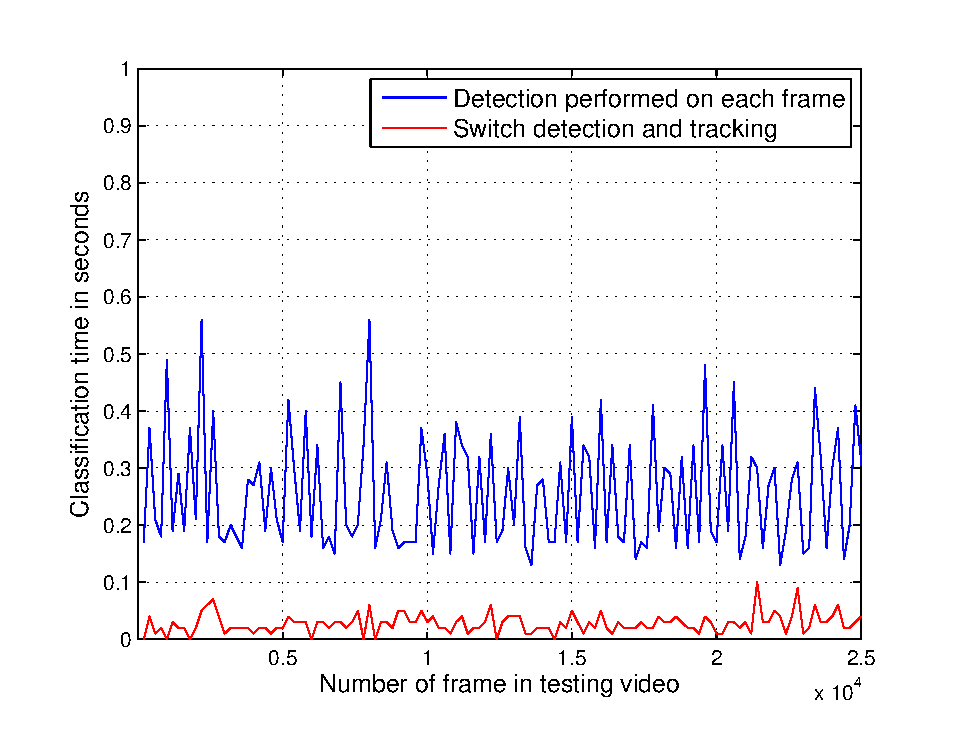
\includegraphics[width=\linewidth]{img/trackingvsdetection.eps}
\caption{Classification time for performing the detection on each
    frame (blue) and switching between detection and tracking (red) along a
    testing video stream}
\label{fig:trackingvsdetection}
\end{figure} 

We test the application on a Samsung S3 GT-I9305 which have a Quad-core 1.4 GHz
Cortex-A9 processor. On the table~\ref{tab:detectionvstracking} are shown the
performance results obtained with the two methods and the average frames per
second using both approaches. Using the mixed strategy push up the frame rate
almost four times.
 
\begin{table}
\begin{tabular}{|c|c|c|c|}
    \hline
    Method & Average running time (sec) & variance & Average FPS \\
    \hline
    Frame-wise detection & $0.1746$ & $7.224 \times 10^4$ & $5.8838$ \\
    \hline
    Detection and tracking  & $0.0555$ & $6.3127 \times 10^5$ & $18.36$ \\
    \hline
\end{tabular}
    \caption{Performance comparison between pure detection and switching between
    detection and tracking}
    \label{tab:detectionvstracking}
\end{table}

An other important comment is that the code was implemented on C++ and executed
by the Android NDK interface. The native code in C++ runs much faster than its
Java counterpart.

% section Performance and running time (end)


